% Load LaTeX and package
\documentclass[11pt, xcolor=x11names,compress]{beamer}
\usepackage[utf8]{inputenc}
\usepackage{mathtools}  % for paired delimiters 
\usepackage{mathrsfs}   % for script capitals
\usepackage{amsmath}
\usepackage{amssymb}
\usepackage{amsfonts}

\usepackage[dvipsnames]{xcolor} % for color
\usepackage{ragged2e} % for text alignment
\usepackage{dsfont} % for sepecial font (mathds)

\usepackage[labelformat=empty]{caption}

\usepackage{threeparttable} 
\usepackage{makecell} 
\usepackage{wrapfig}

\usepackage{natbib}
\bibliographystyle{abbrvnat}
% Customize theme attributes
\setbeamertemplate{headline}[default]
%% Hide navigation symbols
\setbeamertemplate{navigation symbols}{}
%%\mode<beamer>{\setbeamertemplate{blocks}[rounded][shadow=true]} %for block
%% Outer theme
\useoutertheme{infolines}
\useoutertheme[subsection=false]{miniframes}

%% Inner theme
\useinnertheme{}

% Define template colors
\usecolortheme{rose}
%\usecolortheme{default}

% These are my colors -- there are many like them, but these ones are mine.
\definecolor{blue}{RGB}{0,114,178}
\definecolor{red}{RGB}{213,94,0}
\definecolor{yellow}{RGB}{240,228,66}
\definecolor{green}{RGB}{0,158,115}

\definecolor{UniColor}{RGB}{0,0, 255}
\setbeamercolor{structure}{bg=white, fg=UniColor}
\setbeamercolor{title}{bg = white, fg = UniColor}
\setbeamercolor{author}{bg = white, fg = UniColor}

\DeclareMathOperator{\Var}{\text{Var}}
\DeclareMathOperator{\E}{\text{E}}
\DeclareMathOperator{\Cov}{\text{Cov}}
\DeclareMathOperator{\Corr}{\text{Corr}}

%------------------------------------------------------------
%This block of code defines the information to appear in the
%Title page


\title [ECON 4003: Empirical Exercise 4]{ECON 4003 Econometrics I}

\vspace{10mm}

\author[]{Empirical Exercise 4}
\date[]{\textit{By Duong Trinh}}

%End of title page configuration block
%---------------------------------------------------- 

\begin{document}
\setbeamertemplate{caption}[numbered]
%The next statement creates the title page.
{\titlegraphic{
\includegraphics[scale = 0.05]{GlaLogo.pdf}}
\frame{\titlepage}}

%---------------------------------------------------------

\begin{frame}[fragile,t]
\linespread{1.3}
\frametitle{Picture the Scenario}
\begin{itemize}
    \item \textbf{Objective:} Predicting the US presidential elections using economic and political indicators.
    \item \textbf{Dataset:} \texttt{election.dta} 
    \begin{itemize}
        \item [$\square$] which contains 33 observations of elections from 1880 to 2008.
        \item [$\square$] we will use data from 1916 to 2008.
    \end{itemize}
    \item \textbf{Key variables:}
    \begin{itemize}
        \item [$\square$] \texttt{vote}: Percentage share of the popular vote won by the incumbent party
        \item [$\square$] \texttt{growth}: Growth rate of real GDP per capita in the first 3 quarters of the election year
        \item [$\square$] \texttt{inflation}: Inflation rate in the first 15 quarters of the administration period
    \end{itemize}
\end{itemize}
\end{frame}
%---------------------------------------------------------

%---------------------------------------------------------
\begin{frame}[fragile,t]
\frametitle{Question 1} \label{(a1)}
\begin{itemize}
    \item Create a binary variable called majority such that:
$$
\text { majority }=\left\{\begin{array}{l}
1 \text { if votes }>50 \% \\
0 \text { if votes } \leq 50 \%
\end{array}\right.
$$
\item Compare the GDP growth rate per capita for those
incumbents who won with majority and for those who didn’t:
\pause
\vspace{3mm}
\begin{center}
\setlength{\tabcolsep}{3pt}
\begin{tabular}{|l|c|c|c|}
\hline
& All Incumbents & With Majority Vote & Without Majority Vote
\\
\hline
Mean &  1.4129 & 3.3817  & -1.8683 \\
 \hline 
$n$ & 24 & 15 & 9
\\ \hline
\end{tabular}
\end{center}
\vspace{3mm}
The GDP growth rate per capita in the previous 3 quarters of the elections’ year was in average positive with 3.3817\% for those who won with majority and negative with −1.8683\% for those who didn’t win with majority.
\end{itemize}
\end{frame}
%---------------------------------------------------------
%---------------------------------------------------------
\begin{frame}[fragile,t]
\frametitle{Question 2}
Consider the regression model:
$$
vote_i = \beta_0 + \beta_1 growth_i + u_i
$$

\begin{itemize}
    \item (a) Point Estimate  
    \item (b) Hypothesis Testing
    \item (c) Confidence Interval 
\end{itemize}
\end{frame}
%---------------------------------------------------------
%---------------------------------------------------------
\begin{frame}[fragile,t]
\frametitle{Question 2 (a) Point Estimate}
\begin{itemize}
    \item Estimate the regression model:
$$
vote_i = \beta_0 + \beta_1 growth_i + u_i
$$
\pause
Estimation results with heteroskedastic-robust standard errors:
$$\underset{(se)}{\widehat{vote}} = \underset{(1.0658)}{50.8484} +  \underset{(0.1640)}{0.8859} \cdot growth \qquad R^2=0.5189 \quad SER=4.798$$ 
\begin{itemize}
    \item [$\square$] A 1 percentage point increase in the growth rate of real GDP per capita in the 3 quarters before the election \textit{is associated with} a 0.8859 percentage points  increase in the share of votes of the incumbent party \textit{on average}.  \\
    \vspace{2mm}
    \item [$\square$] When real GDP growth is 0, the expected vote of the
    incumbent party is 50.85\% (meaning that it will still maintain the majority vote).
\end{itemize}
\end{itemize}

\end{frame}
%---------------------------------------------------------
%---------------------------------------------------------
\begin{frame}[fragile,t]
\frametitle{Question 2 (b) Hypothesis Testing} 
\begin{itemize}
    \item Test the null hypothesis that economic growth has no effect on the percentage vote earned by the incumbent party at a 5\% significance level.
\end{itemize}
\hyperlink{Hypothesis}{\beamerbutton{Hypothesis}}
\end{frame}
%---------------------------------------------------------

%---------------------------------------------------------
\begin{frame}[fragile,t]
\linespread{1.3}
\frametitle{Question 2 (b) Hypothesis Testing}

Procedure includes 5 steps:
\begin{itemize}
    \item Null hypothesis $H_0$
    \item Alternative hypothesis $H_1$
    \item Test statistic
    \item Decision rule
    \item Conclusion
\end{itemize}

\end{frame}
%---------------------------------------------------------

%---------------------------------------------------------
\begin{frame}[fragile,t]
\frametitle{Question 2 (b) Hypothesis Testing} 
\linespread{1.15}
\begin{itemize}
    \item [$\blacksquare$] Null hypothesis $H_0$:
    \begin{itemize}
        \item [$\square$] $H_0$: GDP growth has no effect on the percentage vote\\
              $H_0: \beta_1 = 0$
    \end{itemize}
    \item Alternative hypothesis $H_1$
    \item Test statistic
    \item Decision rule
    \item Conclusion
\end{itemize}
\end{frame}
%---------------------------------------------------------
%---------------------------------------------------------
\begin{frame}[fragile,t]
\frametitle{Question 2 (b) Hypothesis Testing} 
\linespread{1.15}
\begin{itemize}
    \item [$\blacksquare$] Null hypothesis $H_0$:
    \begin{itemize}
        \item [$\square$] $H_0$: GDP growth has no effect on the percentage vote\\
              $H_0: \beta_1 = 0$
    \end{itemize}
    \item [$\blacksquare$] Alternative hypothesis $H_1$:
    \begin{itemize}
        \item [$\square$] $H_1$: GDP growth has a positive effect on the percentage of vote\\
              $H_1: \beta_1 > 0$
        \item [$\square$] We take the assumption that when the economy is doing well, the incumbent party has a better chance to win the elections.  
    \end{itemize}    
    \item Test statistic
    \item Decision rule
    \item Conclusion
\end{itemize}
\end{frame}
%---------------------------------------------------------
%---------------------------------------------------------
\begin{frame}[fragile,t]
\frametitle{Question 2 (b) Hypothesis Testing} 
\linespread{1.15}
\begin{itemize}
    \item Null hypothesis $H_0$
    \item Alternative hypothesis $H_1$
    \item [$\blacksquare$] Test statistic:
$$
\text{t-statistic}=\frac{\hat{\beta}_{1}-0}{S E\left(\hat{\beta}_{1}\right)}=\frac{0.8859-0}{0.1640}=5.40
$$    \item Decision rule
    \item Conclusion
\end{itemize}
\end{frame}
%---------------------------------------------------------
%---------------------------------------------------------
\begin{frame}[fragile,t]
\frametitle{Question 2 (b) Hypothesis Testing} 
\linespread{1.15}
\begin{itemize}
    \item [$\blacksquare$] Test statistic:
$$
\text{t-statistic}=\frac{\hat{\beta}_{1}-0}{S E\left(\hat{\beta}_{1}\right)}=\frac{0.8859-0}{0.1640}=5.40
$$   
\end{itemize}
\begin{figure}
    \centering
    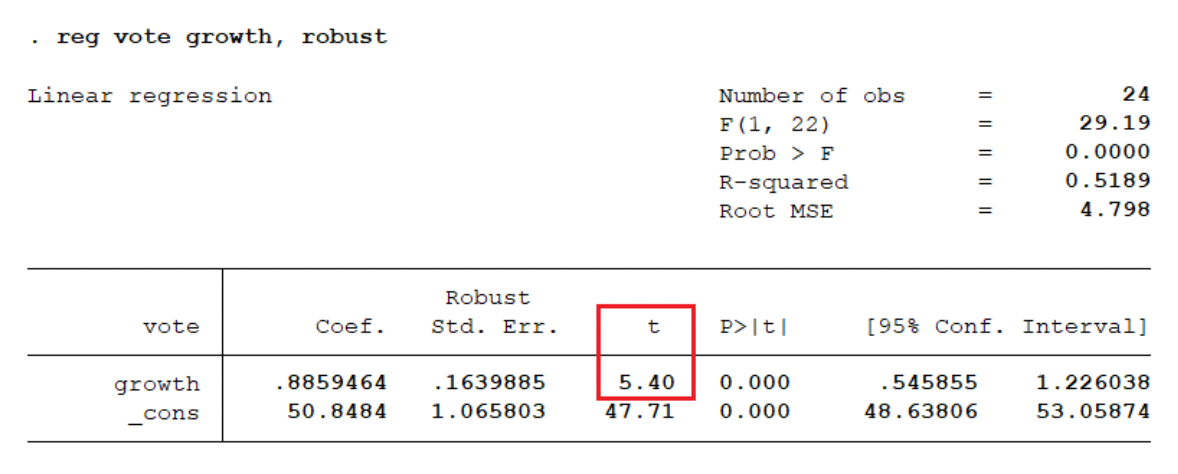
\includegraphics[scale = 0.55]{Q2_tstat.png}
    \caption{}
\end{figure}
\end{frame}
%---------------------------------------------------------
%---------------------------------------------------------
\begin{frame}[fragile,t]
\frametitle{Question 2 (b) Hypothesis Testing} 
\linespread{1.15}
\begin{itemize}
    \item Null hypothesis $H_0$
    \item Alternative hypothesis $H_1$
    \item Test statistic
    \item [$\blacksquare$] Decision rule:
    \begin{itemize}
        \item [$\square$] Is this a two-sided test or an one-sided (left-tailed/right-tailed) test?\\
        $\Longrightarrow$ Right-tailed test (Look again $H_1: \beta_1 > 0$).
        \item [$\square$] What is the \textbf{significance level} $\alpha$?\\
        $\Longrightarrow$ $5\%$ significance level.
        \item [$\square$] Is the decision rule based on \textcolor{green}{\textbf{critical values}} or \textcolor{red}{\textbf{p-value}}?\\
        $\Longrightarrow$ Distinguish...
    \end{itemize}
    \item Conclusion
\end{itemize}

\end{frame}
%---------------------------------------------------------
%---------------------------------------------------------
\begin{frame}[fragile,t]
\frametitle{Question 2 (b) Hypothesis Testing} 
\linespread{1.15}
\begin{itemize}
    \item [$\blacksquare$] Decision rule:
    \begin{itemize}
        \item [$\square$] Right-tailed test 
        \item [$\square$] The significance level $\alpha = 0.05$
        \item [$\square$] Is the decision rule based on \textcolor{green}{\textbf{critical values}} or \textcolor{red}{\textbf{p-value}}?\\
        \vspace{2mm}
        \textcolor{green}{*Approach 1: \textbf{Critical-value Test}:} Reject $H_0$ if t-statistic $> t_{\alpha,n-2}$
        \begin{itemize}
            \item The critical value is: $t_{0.05,22} = 1.7171$ \\
            \vspace{2mm}
            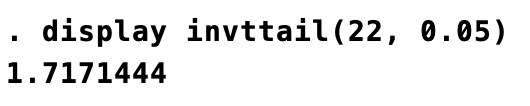
\includegraphics[scale = 0.5]{CriticalValue.png}
            \vspace{3mm}
            \item Since $5.40 > 1.7171$, we \textit{reject }$H_0$ at 5\% level of significance.
            \end{itemize}
    \end{itemize}
\end{itemize}
\end{frame}
%---------------------------------------------------------
%---------------------------------------------------------
\begin{frame}[fragile,t]
\frametitle{Question 2 (b) Hypothesis Testing} 
\linespread{1.15}
\begin{itemize}
    \item [$\blacksquare$] Decision rule:
    \begin{itemize}
        \item [$\square$] Right-tailed test 
        \item [$\square$] The significance level $\alpha = 0.05$
        \item [$\square$] Is the decision rule based on \textcolor{green}{\textbf{critical values}} or \textcolor{red}{\textbf{p-value}}?\\
        \vspace{2mm}
     \textcolor{red}{*Approach 2: \textbf{P-value Test}:} Reject $H_0$ if P-value $\leq \alpha$
        \begin{itemize}
            \item Stata displays by default a two-sided p value:\\
            p-value one-sided = p-value two-sided/2 $\approx 0.000$ 
            \item Since $0.000 < 0.05 = \alpha$, we reject $H_0$ at 5\% level of significance.
        \end{itemize}
    \vspace{2mm}
    \begin{figure}
        \centering
    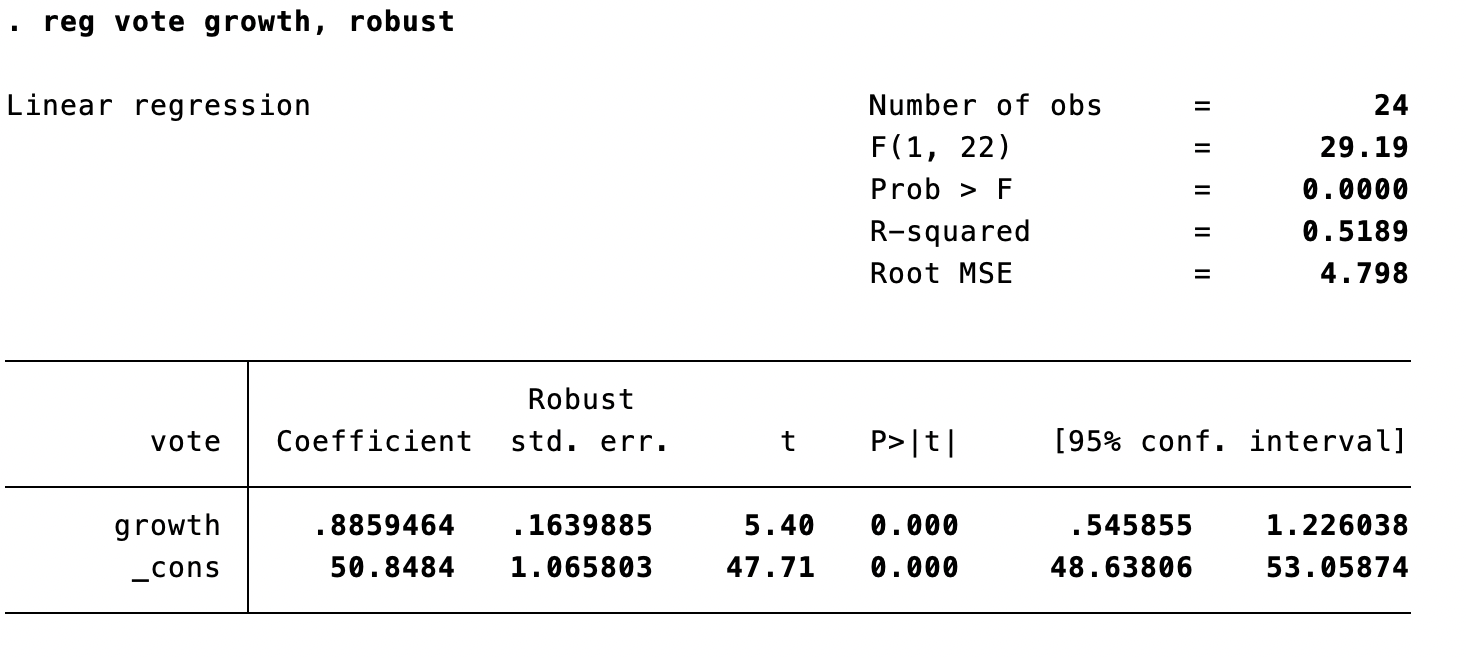
\includegraphics[scale = 0.3]{P-value.png}
        \caption{}
    \end{figure}
\end{itemize}

\end{itemize}
\end{frame}
%---------------------------------------------------------
%---------------------------------------------------------
\begin{frame}[fragile,t]
\frametitle{Question 2 (b) Hypothesis Testing} 
\linespread{1.15}
\begin{itemize}
    \item Null hypothesis $H_0$
    \item Alternative hypothesis $H_1$
    \item Test statistic
   \item Decision rule
    \item [$\blacksquare$] Conclusion:
    \begin{itemize}
        \item [$\square$] Real GDP growth rate per capita has a significant positive effect relation with the percentage votes of the incumbent
party.
    \end{itemize}
\end{itemize}
\end{frame}
%---------------------------------------------------------

%---------------------------------------------------------
\begin{frame}[fragile,t]
\frametitle{Question 2 (c) Confidence Interval} 
\linespread{1.15}
\begin{itemize}
    \item What is the 95\% confidence interval for  $\beta_1$? Interpret the result. What are the 90\% and 99\% confidence intervals for $\beta_1$?
\end{itemize}
\hyperlink{CIs}{\beamerbutton{CIs}}
\end{frame}
%---------------------------------------------------------

%---------------------------------------------------------
\begin{frame}[fragile,t]
\frametitle{Question 2 (c) Confidence Intervals} 
\linespread{1.15}
\begin{itemize}
    \item The 95\% confidence interval for  $\beta_1$ is
$$
\left[\widehat{\beta}_{1} - t_{\frac{0.05}{2}, 22} \cdot S E\left(\widehat{\beta}_{1}\right),\widehat{\beta}_{1} + t_{\frac{0.05}{2}, 22} \cdot SE\left(\widehat{\beta}_{1}\right)\right]
$$
\begin{figure}
    \centering
    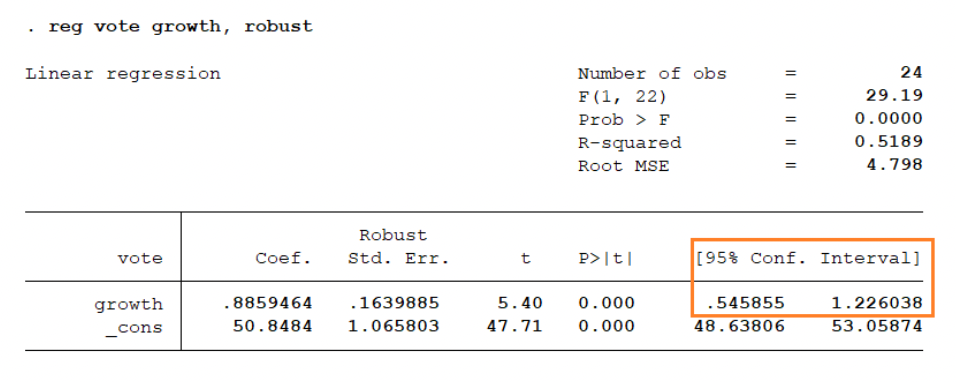
\includegraphics[scale = 0.65]{Q2_95CI.png}
\end{figure}
    \item By default Stata displays the 95\% Confidence Interval which is $[0.5459; .2260]$
\end{itemize}
\end{frame}
%---------------------------------------------------------

%---------------------------------------------------------
\begin{frame}[fragile,t]
\frametitle{Question 2 (c) Confidence Intervals} 
\linespread{1.3}
\begin{itemize}
    \item The 95\% confidence interval for  $\beta_1$ is
$$
[0.5459; 1.2260]
$$
    \item In repeated samples, 95\% of the intervals constructed in this way will contain the true value of parameter $\beta_1$.
    \item The lower bound of the 95\% Confidence Interval is positive, referring that GDP growth rate and the share of votes for the incumbent party have a positive relationship.
\end{itemize}
\end{frame}
%---------------------------------------------------------

%---------------------------------------------------------
\begin{frame}[fragile,t]
\frametitle{Question 2 (c) Confidence Intervals} 
\linespread{1.15}
\begin{itemize}
    \item The 90\% confidence interval for  $\beta_1$ is
$$
\left[\widehat{\beta}_{1} - t_{\frac{0.1}{2}, 22} \cdot S E\left(\widehat{\beta}_{1}\right),\widehat{\beta}_{1} + t_{\frac{0.1}{2}, 22} \cdot SE\left(\widehat{\beta}_{1}\right)\right]
$$
\begin{figure}
    \centering
    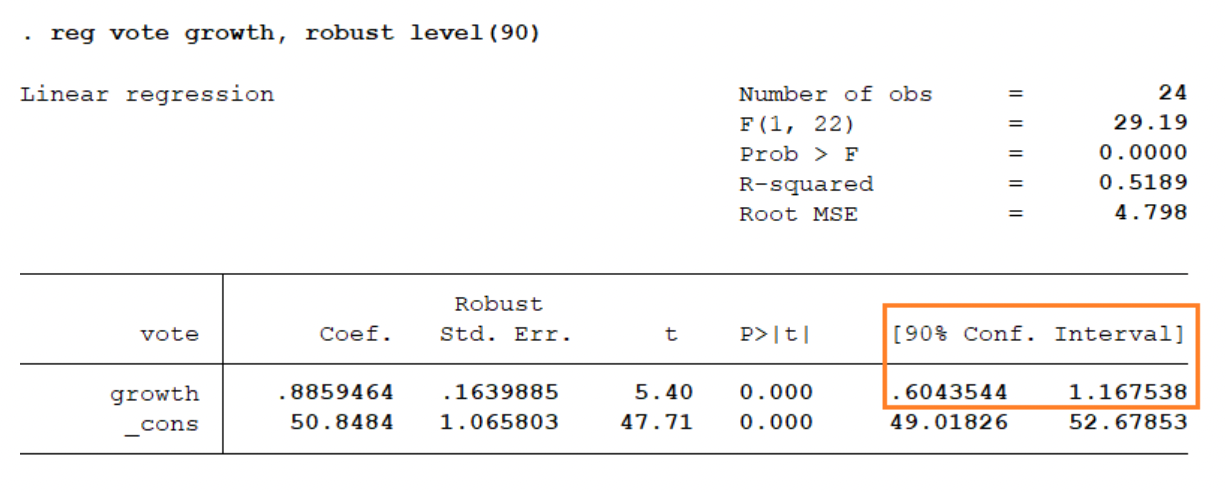
\includegraphics[scale = 0.5]{Q2_90CI.png}
\end{figure}
\end{itemize}
\end{frame}
%---------------------------------------------------------

%---------------------------------------------------------
\begin{frame}[fragile,t]
\frametitle{Question 2 (c) Confidence Intervals} 
\linespread{1.15}
\begin{itemize}
    \item The 99\% confidence interval for  $\beta_1$ is
$$
\left[\widehat{\beta}_{1} - t_{\frac{0.01}{2}, 22} \cdot S E\left(\widehat{\beta}_{1}\right),\widehat{\beta}_{1} + t_{\frac{0.01}{2}, 22} \cdot SE\left(\widehat{\beta}_{1}\right)\right]
$$
\begin{figure}
    \centering
    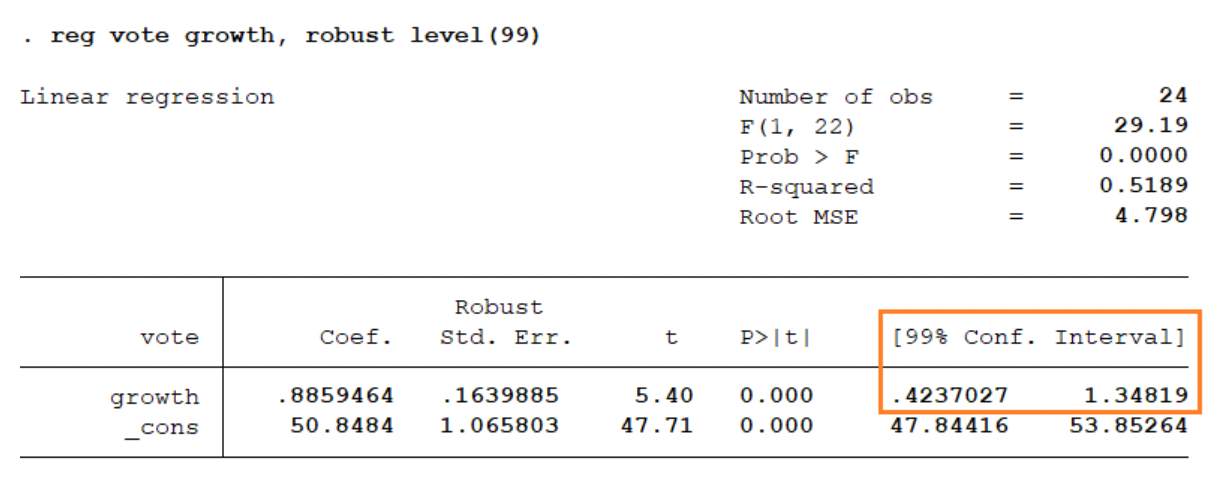
\includegraphics[scale = 0.5]{Q2_99CI.png}
\end{figure}
\end{itemize}
\end{frame}
%---------------------------------------------------------

%---------------------------------------------------------
\begin{frame}[fragile,t]
\frametitle{Question 3}
Estimate the regression model:
$$
vote_i = \gamma_0 + \gamma_1 inflation_i + u_i
$$

\begin{itemize}
    \item (a,b) Test the null hypothesis that inflation has no effect on the percentage vote earned by the incumbent party at a 1\% significance level.
    \item (c) Test the null hypothesis that if inflation is zero the expected vote in favour of the incumbent party is 50\% or more at a 1\% significance level.
\end{itemize}
\end{frame}
%---------------------------------------------------------

%---------------------------------------------------------
\begin{frame}[fragile,t]
\frametitle{Question 3 (c)}
\linespread{1.15}
Hypothesis testing for the expected vote when inflation is 0
$$
\mathbb{E}\left[vote_i \mid inflation_i =0\right]=\gamma_{0}+\gamma_{1} \times 0=\gamma_{0}
$$
\begin{itemize}
    \item [$\blacksquare$] Null hypothesis $H_0$:
    \begin{itemize}
        \item [$\square$] $H_0$: Expected vote of the incumbent is 50\% or more\\
              $H_0: \gamma_0 \geq 50\%$
    \end{itemize}
    \item [$\blacksquare$] Alternative hypothesis $H_1$:
    \begin{itemize}
        \item [$\square$] $H_1$: Expected vote of the incumbent lower than 50\%\\
              $H_1: \gamma_0 < 50\%$
    \end{itemize}    
    \item Test statistic
    \item Decision rule
    \item Conclusion
\end{itemize}
\end{frame}
%---------------------------------------------------------

%---------------------------------------------------------
\begin{frame}[fragile,t]
\frametitle{Testing Hypotheses About One
of Regression Coefficients}\label{Hypothesis}
\linespread{1.3}
\begin{itemize}
    \item $\beta_1$ are \textbf{unknown} features of the population (population parameters), and we will never know them with certainty.
    \item Nevertheless, we can \textbf{hypothesize} about the value of $\beta_1$ and then use statistical inference to test our hypothesis.
\end{itemize}
 \end{frame}
%---------------------------------------------------------

%---------------------------------------------------------
\begin{frame}[fragile,t]
\linespread{1.3}
\frametitle{Testing Hypotheses About One
of Regression Coefficients}

Procedure includes 5 steps:
\begin{itemize}
    \item Null hypothesis $H_0$
    \item Alternative hypothesis $H_1$
    \item Test statistic
    \item Decision rule
    \item Conclusion
\end{itemize}

\end{frame}
%---------------------------------------------------------

%---------------------------------------------------------
\begin{frame}[fragile,t]
\linespread{1.15}
\frametitle{Testing Hypotheses About One
of Regression Coefficients}

Procedure includes 5 steps:
\begin{itemize}
    \item [$\blacksquare$] Null hypothesis $H_0$:\\
    $$
    H_0: \beta_1 = \beta_{1,0}
    $$
    where $\beta_{1,0}$ is a hypothesized value.
    \item Alternative hypothesis $H_1$
    \item Test statistic
    \item Decision rule
    \item Conclusion
\end{itemize}

\end{frame}
%---------------------------------------------------------

%---------------------------------------------------------
\begin{frame}[fragile,t]
\linespread{1.15}
\frametitle{Testing Hypotheses About One
of Regression Coefficients}

Procedure includes 5 steps:
\begin{itemize}
    \item [$\blacksquare$] Null hypothesis $H_0$:\\
    $$
    H_0: \beta_1 = \beta_{1,0}
    $$
    where $\beta_{1,0}$ is a hypothesized value.
    \item [$\blacksquare$] Alternative hypothesis $H_1$:
    \vspace{2mm}
    \begin{center}
    \begin{tabular}{|c|c|}
    \hline
    Test & $H_1$\\
    \hline
    Two-sided &  \beta_1 \neq \beta_{1,0} \\
    \hline 
    Left-tailed & \beta_1 < \beta_{1,0}\\
    \hline 
    Right-tailed & \beta_1 > \beta_{1,0}\\ 
    \hline
    \end{tabular}
    \end{center}
    \vspace{2mm}
    \item Test statistic
    \item Decision rule
    \item Conclusion
\end{itemize}

\end{frame}
%---------------------------------------------------------
%---------------------------------------------------------
\begin{frame}[fragile,t]
\linespread{1.15}
\frametitle{Testing Hypotheses About One
of Regression Coefficients}

Procedure includes 5 steps:
\begin{itemize}
    \item Null hypothesis $H_0$
    \item Alternative hypothesis $H_1$
    \item [$\blacksquare$] Test statistic:
    $$
    \textbf{\text{t-statistic}} =\frac{\widehat{\beta}_{1}-\beta_{1,0}}{S E\left(\widehat{\beta}_{1}\right)}
    $$
    follows a t-distribution with degrees of freedom $n-2$ 
    \item Decision rule
    \item Conclusion
\end{itemize}

\end{frame}
%---------------------------------------------------------

%---------------------------------------------------------
\begin{frame}[fragile,t]
\linespread{1.15}
\frametitle{Testing Hypotheses About One
of Regression Coefficients}

Procedure includes 5 steps:
\begin{itemize}
    \item Null hypothesis $H_0$
    \item Alternative hypothesis $H_1$
    \item Test statistic
    \item [$\blacksquare$] Decision rule:
    \begin{itemize}
        \item [$\square$] Is this a two-sided test or an one-sided (left-tailed/right-tailed) test?\\
        $\Longrightarrow$ Look again $H_1$.
        \item [$\square$] What is the \textbf{significance level} $\alpha$?\\
        $\Longrightarrow$ Usually chosen to be 0.01, 0.05 or 0.10.
        \item [$\square$] Is the decision rule based on \textcolor{green}{\textbf{critical values}} or \textcolor{red}{\textbf{p-value}}?\\
        $\Longrightarrow$ Distinguish...
    \end{itemize}
    \item Conclusion
\end{itemize}

\end{frame}
%---------------------------------------------------------

%---------------------------------------------------------
\begin{frame}[fragile,t]
\linespread{1.15}
\frametitle{Decision Rule}
    \begin{center}
    Approach 1: \textcolor{green}{\textbf{Critical-value Test}}\\
    \vspace{3mm}
    \begin{tabular}{|c|c|c|}
    \hline
    Test & $H_1$ & Reject $H_0$ if\\
    \hline
    Two-sided &  \beta_1 \neq \beta_{1,0} & $ t^s < -t_{\frac{\alpha}{2}}$ or $ t^s> t_{\frac{\alpha}{2}}$\\
    \hline 
    Left-tailed & \beta_1 < \beta_{1,0} & $t^s < - t_{\alpha}$\\ 
    \hline 
    Right-tailed & \beta_1 > \beta_{1,0} & $t^s > t_{\alpha}$\\ 
    \hline
    \end{tabular}
    \end{center}
    
    \vspace{4mm}
    
    \begin{center}
    Approach 2: \textcolor{red}{\textbf{p-value Test}}\\
    \vspace{3mm}
    \begin{tabular}{|c|c|c|c|}
    \hline
    Test & $H_1$ & p-value & Reject $H_0$ if\\
    \hline
    Two-sided &  \beta_1 \neq \beta_{1,0} & \makecell{sum probabilities to the right \\ of $|t^s|$ and to the left of $-|t^s|$} & p-value $\leq \alpha$\\
    \hline 
    Left-tailed & \beta_1 < \beta_{1,0} & probability to the left of $t^s$ & p-value $\leq \alpha$\\ 
    \hline 
    Right-tailed & \beta_1 > \beta_{1,0} & probability to the right of $t^s$ & p-value $\leq \alpha$\\ 
    \hline
    \end{tabular}
    
    \vspace{1mm}
    
    *Note: p-value two-sided = 2 × p-value one-sided 
    \end{center}
\end{frame}
%---------------------------------------------------------

%---------------------------------------------------------
\begin{frame}[fragile,t]
\frametitle{Decision Rule}
\begin{figure}
    \centering
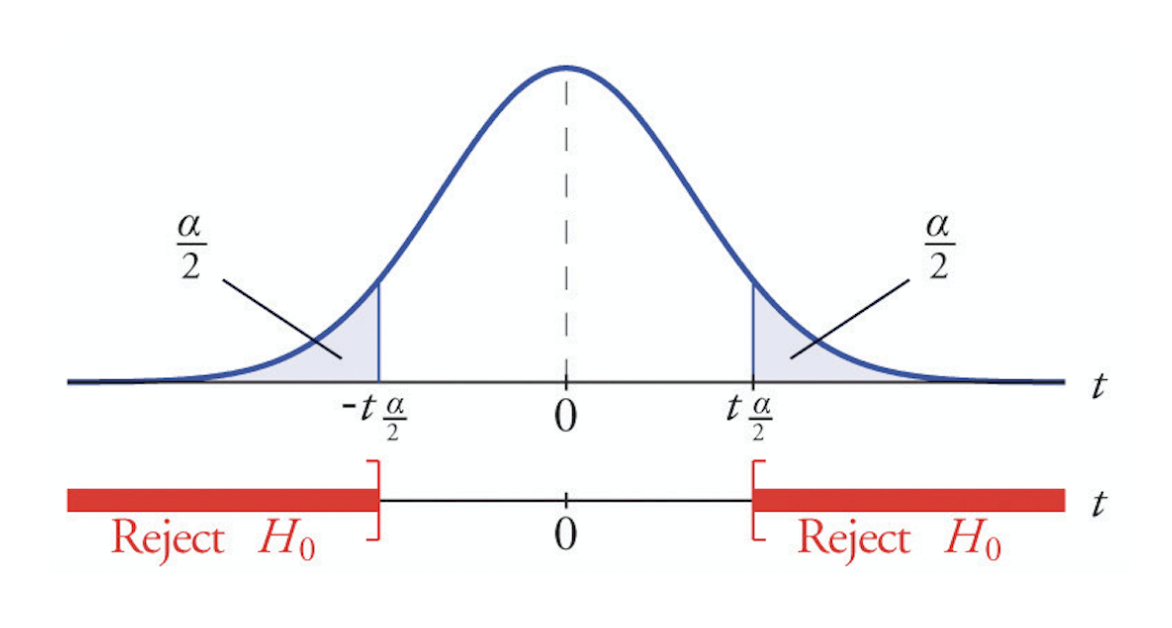
\includegraphics[scale = 0.29]{two-sided.png}\\
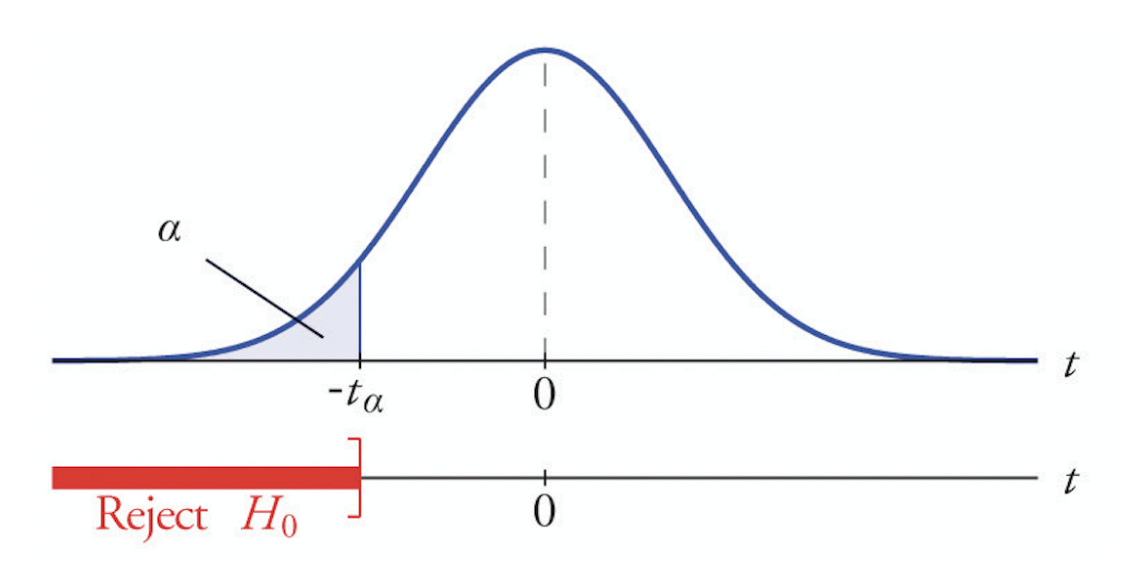
\includegraphics[scale = 0.29]{left-tailed.png}
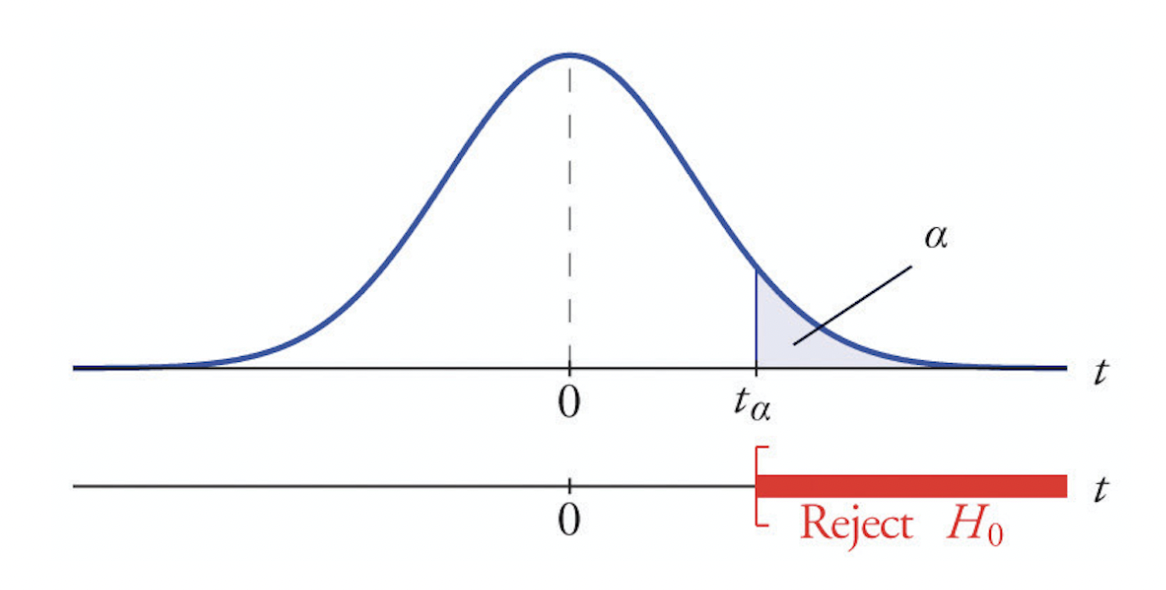
\includegraphics[scale = 0.29]{right-tailed.png}
    \caption{}
\end{figure}

\end{frame}
%---------------------------------------------------------

%---------------------------------------------------------
\begin{frame}[fragile,t]
\linespread{1.3}
\frametitle{Testing Hypotheses About One
of Regression Coefficients}

Procedure includes 5 steps:
\begin{itemize}
    \item Null hypothesis $H_0$
    \item Alternative hypothesis $H_1$
    \item Test statistic
    \item Decision rule
    \item [$\blacksquare$] Conclusion:
    \begin{itemize}
        \item [$\square$] Do you \textit{reject} or or \textit{fail to reject} the null hypothesis at the significance level $\alpha$?
        \item [$\square$] AVOID saying that you "\textit{accept}" the null hypothesis, which can be very misleading
    \end{itemize}
\end{itemize}
\end{frame}
%---------------------------------------------------------
%---------------------------------------------------------
\begin{frame}[fragile,t]
\frametitle{Confidence Intervals}\label{CIs}
\linespread{1.15}
\begin{itemize}
\item The $100(1-\alpha)\%$ confidence interval for $\beta_1$ is given by
$$
\left[\widehat{\beta}_{1} - t_{\frac{\alpha}{2}, n-2} \cdot S E\left(\widehat{\beta}_{1}\right), \widehat{\beta}_{1} + t_{\frac{\alpha}{2}, n-2} \cdot S E\left(\widehat{\beta}_{1}\right) \right]
$$
\begin{itemize}
    \item [$\square$] Usually $\alpha = 0.01, 0.05$ or $0.10$, so that we obtain a 99\%, 95\% or 90\% confidence interval, respectively.
    \vspace{2mm}
    \item [$\square$] $t_{\frac{\alpha}{2}, n-2}:$ same critical value as two-sided hypothesis test.
\end{itemize}
\end{itemize}
 \end{frame}
%---------------------------------------------------------
%---------------------------------------------------------
\begin{frame}[fragile,t]
\frametitle{Confidence Intervals}
\begin{figure}
    \centering
    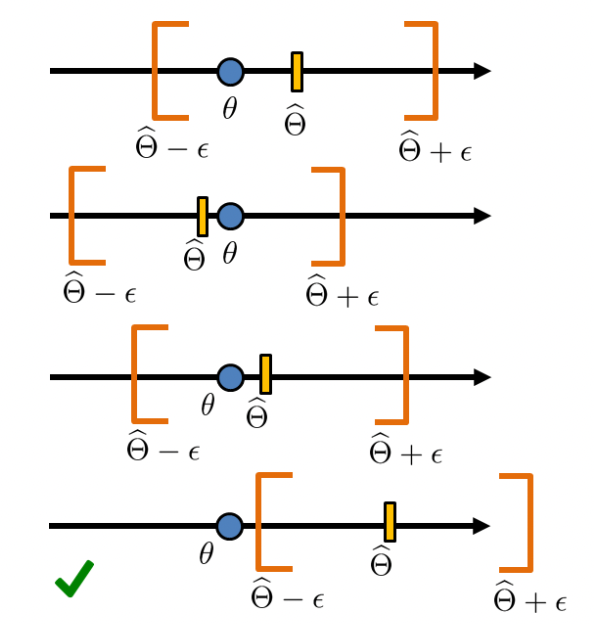
\includegraphics[scale = 0.5]{VisualCIs.png}
    \caption{If you have 100 random realizations of the confidence intervals, then 95 on average will include the true parameter.}
\end{figure}
 \end{frame}
%---------------------------------------------------------
%---------------------------------------------------------
\end{document}